\documentclass{article}[12pt]
\usepackage{amsmath}
\usepackage{graphicx}
\usepackage{verbatim}
\usepackage{fullpage}
\begin{document}

\thispagestyle{empty}
\pagestyle{plain}

\author{Adin Scannell}
\title{SMACHE: Space-efficient Caching for Self-Similar Data}
\maketitle

\section{Introduction}

Scientific applications are on the verge of generating enough data to overwhelm
existing computing paradigms.  For example, next generation sequencing
technology from Applied Biosystems, SOLiD, generates approximately 1 terabyte
of image data every run~\cite{ab}.  In this magnitude, data rapidly overwhelms
any individual system and must be processed by a distributed system.

Manually managing and distributing data to a distributed application is too
complex and burdensome for a programmer.  New programming frameworks such as
Map-Reduce reverse the relationship between data and computation on a cluster.
Instead of moving data to a processing element, logic and computation move to
the data and execute where it resides.

Unfortunately, long-lived computations may require several pieces of data
simultaneously and it may not be possible to schedule a computation near
everything it needs.  For example, it may not be possible to schedule an
application that compares the genome from human $A$ and the genome from human
$B$ on a node where both genomes are available.  Thus, even a data-centric
paradigm such as Map-Reduce does not completely eliminate the need to move
data.

We believe that SnowFlock~\cite{snowflock} is a useful paradigm for simplifying
cluster computing.  SnowFlock allows programmers to fork Virtual Machine (VM)
instances to create new compute instances.  New VMs may still be scheduled and
moved near data in order to minimize the cost of accessing the large data sets
that the program needs.  In SnowFlock however, more flexibility is given to the
programmer.

In general, both data-centric paradigms such as Map-Reduce and hybrid paradigms
such as SnowFlock require efficient data {\em and} computation transport.  We
can we reduce (but not eliminate) the amount of data that must moved by moving
some of the compute logic.  VM data and biological data have much more in
common than it would seem at a cursory glance; both are simply program
specifications\footnote{A humorous bit of oversimplification.}.  Both share
the same tendency to have internal repetition and self-similarity as well as
similarity to other biological data or VM images.  For example: similar snippets
of code and data frequently repeat in both genomes~\cite{biosequence} and
different programs on a disk.  Similarly, genomes from different members of the
same species are largely similar with only small mutations just as different
versions of a Debian disk image are similar.

This project aims to provide space-efficient caching of data exhibiting
high-levels of self-similarity using techniques similar to those employed by
remote differential compression~\cite{rdc} (RDC).  These techniques have been
applied successfully to {\em significantly} reduce the amount of data required
to synchronize large collections of files over a network~\cite{improvedfile},
but they also have applicability for maintaining efficient caches for cluster
computing.  These caches would similarly allow for efficient data replication
across the network.  As far as I know, they have not been applied in this
context before.  In both SnowFlock and paradigms such as Map-Reduce, caching is
necessarily used to ensure that the costs of transferring data and computation
between nodes is minimized.

\section{Insight and Design}
\label{sec:insight}

Several protocols exist for efficiently transferring data from a remote site
when {\em partial} information already exists locally.  A famous example of
such a protocol is {\tt rsync}~\cite{rsync}.  Whilst {\tt rsync} is dependent
on specific files, protocols such as RDC~\cite{rdc} leverage the fact that
several files may contain similar data or that names may have changed.

We propose to use techniques similar to those employed by RDC in order to
store data exhibiting self-similarity efficiently.  A brief description of
these techniques is included here.

\subsection*{Content-Sensitive Block Algorithms}

A key insight of RDC is the use of a content-sensitive block algorithms.  When
data is added to the cache, it is divided up in a set of blocks.  As opposed to
chunking up data into fixed-size pieces, the pieces are computed as a function
of the data itself.  For example, consider the following DNA sequence:
\begin{center}
AGCGCCAATTAGCTAGCTATGCAATTAGCATTTAGCTAGCT
\end{center}
If we divide in fixed chunks we end up with:
\begin{center}
AGCGC, CAATT, AGCTA, GCTAT, GCAAT, TAGCA, TTTAG, CTAGC, T
\end{center}
Which has no repeated blocks.  However, if we use a content-sensitive block
algorithms, such as splitting at every pair {\tt TA}, we have:
\begin{center}
AGCGCCAATT, AGCTAGCT, ATGCAATT, AGCATTT, AGCTAGCT
\end{center}
In this case, the sequence {\tt AGCTAGCT} is repeated in this genome, and does
not need to be stored twice.

To provide further motivation, consider the above DNA sequence with a single
base-pair inserted at the beginning:
\begin{center}
TAGCGCCAATTAGCTAGCTATGCAATTAGCATTTAGCTAGCT
\end{center}
A fixed-side block algorithm would divide this into:
\begin{center}
TAGCG, CCAAT, TAGCT, AGCTA, TGCAA, TTAGC, ATTTA, GCTAG, CT
\end{center}
Which shares few blocks with the first fixed-block sequence.  However, the
content-sensitive block algorithm described above would divide the sequence
into:
\begin{center}
TAGCGCAATT, AGCTAGCT, ATGCAATT, AGCATTT, AGCTAGCT
\end{center}
This sequence shares all blocks with the first sequence except the first
(modified) block.  Thus to store both the first and second sequence, we need
only store 5 unique blocks.

In reality, no a priori distribution of content is assumed.  The
block-splitting algorithm is run over a sequence generated by taking a Rabin
hash over a sliding window~\cite{rabin}.  After splitting a sequence, each
block may be represented by a key such as a block-hash.  To store a set of
sequences in the cache, one needs only store the sequence of block-hashes and
the set of all {\em unique} blocks.  Information regarding specific
block-splitting and block-hashing algorithms are omitted for brievity.

By storing only unique blocks and sending data as sequences of block-hashes,
SMACHE intends to achieve significant savings for data that exhibits a
high-degree of self-similarity.  There is an interesting tradeoff associated
with the size of the blocks.  Given smaller blocks, hashes impose more
overhead.  However, smaller blocks increase potential savings due to repeated
sequences.  A key challenge in the design of the system will be the evaluation
of system parameters such as {\em mean block size}.

\subsubsection{Goals}
\label{sec:goals}

Biological data shows a high degree of self similarity, which has been used
effectively to compress far beyond 2 bits per base-pair~\cite{biosequence}.
Such similarity may come from shared genes or even common subsequences within a
single genome such as promoters.  Similar techniques have been applied to
running VMs, which also exhibit high degrees of self-similarity, primarily for
the purpose of fitting more running VMs into a smaller amount of
memory~\cite{difference-engine}.

The aim of this project is to provide speed on par with or faster than standard
compression techniques such as Lempel-Ziv, with random access semantics, unlike
Lempel-Ziv.  We do not expect to beat compression ratios achieved by standard
compression algorithms, however we do expect to see significant gains over a
flat cache.

This caching system can be used in two practical scenarios.  First, on a
cluster where the goal is to reduce the time to access data as much as
possible.  In this case, the bottleneck might be disk access; SMACHE may store
its cache database in a distributed-memory system such as
memcached~\cite{memcached}.  Second, if the network bandwidth or latency is a
limiting factor.  This might be the case if a VM or dataset is remote; SMACHE
may use a backing store such as BerkeleyDB~\cite{berkeleydb}.

We believe that there is an attractive opportunity to compress biological data
for caching purposes.  Often in theoretical treatments of compression of
biological data, performance is explicitly not given any
regard~\cite{statistical}.  However, no gains may be made by compression
techniques if the computation cost is so high that data is generated faster
than data can be compressed.  The proposed technique should impose only
moderate overhead.

Additionally, we hope to take advantage of the similarity {\em between}
sequences and VM images for gains in space-efficiency, something which is often
not done in practice.  The possible gains of zipping a single VM image or
biological sequence are severely limited compared to those that can be made by
compressing a set together.  The reason that this does not happen using
existing compression algorithm algorithms is because they often do not offer
random access semantics, i.e. if one compresses ten sequences together then it
is often necessary to extract all ten before extracting the last one.  This is
simply due to the nature of many compression algorithms.

\section{Implementation}
\label{sec:implementation}

This intention of this project is to construct a useful building block on which
future cloud computing tools and infrastructure may be based.  Thus the primary
output will be a simple shared library, {\tt libsmache}, which provides simple
access to cached and uncached data using client and server semantics.

\begin{figure}
\begin{center}
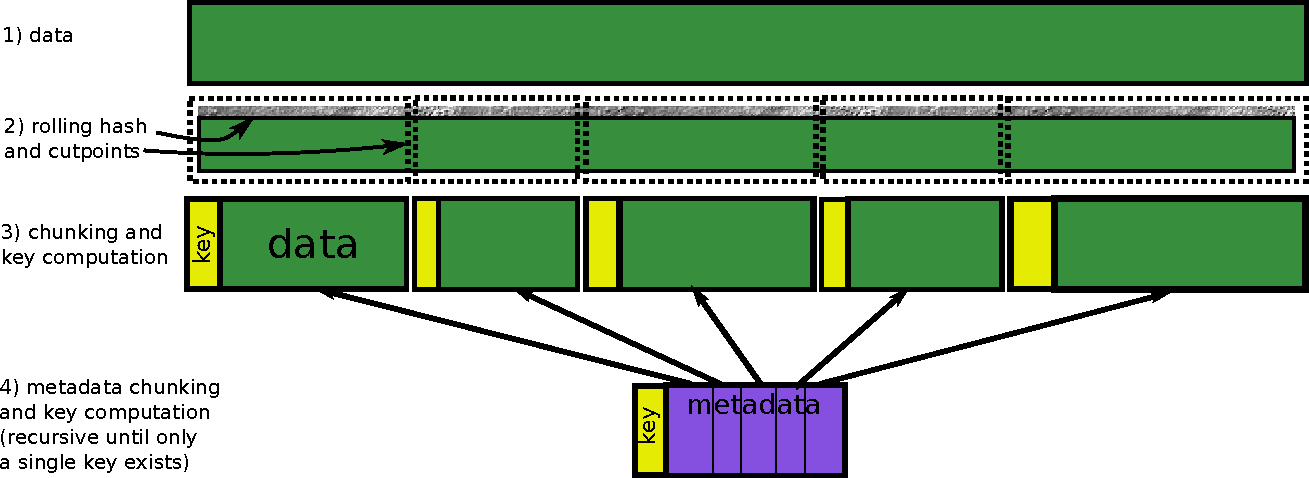
\includegraphics[width=5.5in]{algo}
\caption{The algorithm used for storing data.}
\label{fig:algo}
\end{center}
\end{figure}

A simple utility {\tt smachezip} will be built on top of this shared library,
which given a set of binary data will construct or extract a cache.  This is
tool which will be used to evaluate the effectiveness of the cache.

\begin{figure}
\begin{center}
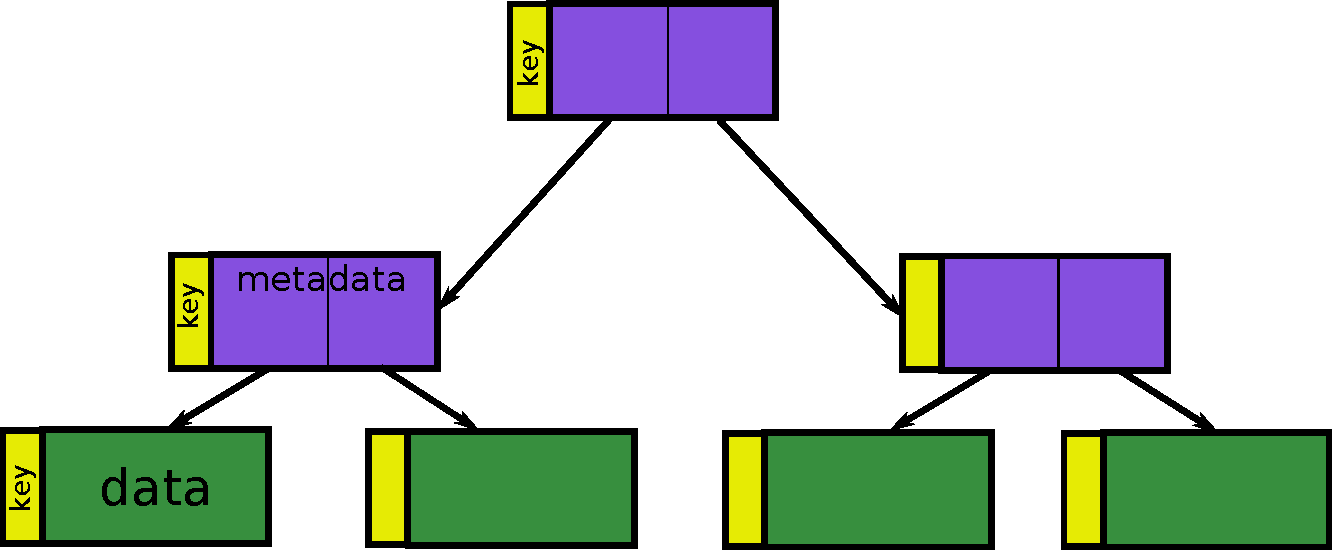
\includegraphics[width=5.5in]{tree}
\caption{An example data tree.}
\label{fig:tree}
\end{center}
\end{figure}

\section{Evaluation}
\label{sec:evaluation}

\begin{figure}
\begin{center}
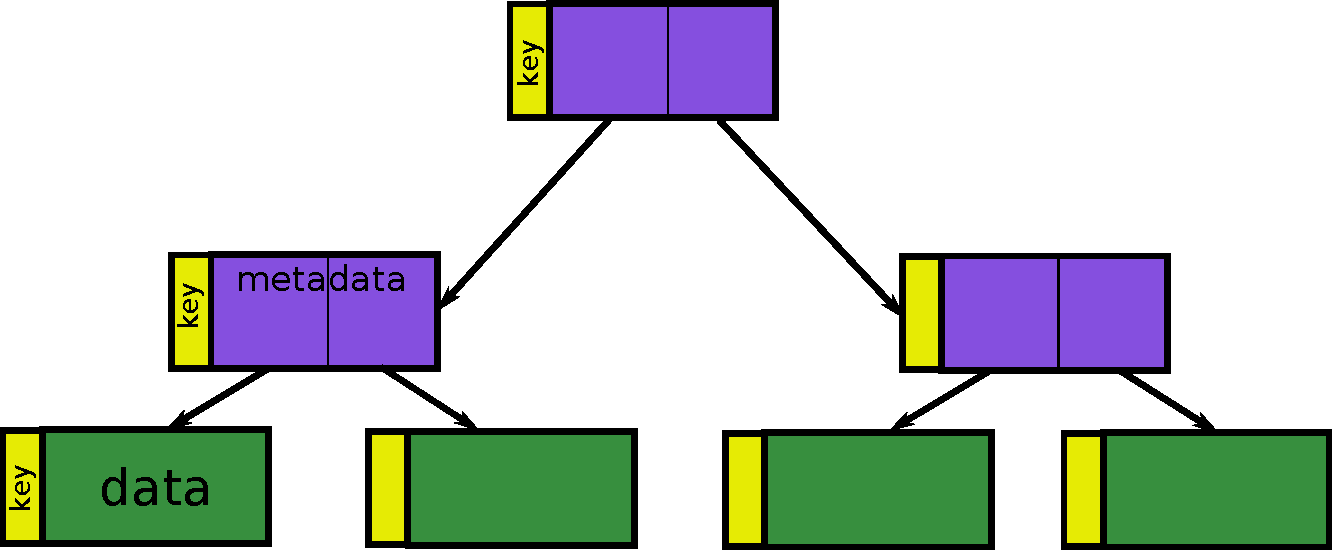
\includegraphics[width=5.5in]{tree}
\caption{An example data tree.}
\label{fig:tree}
\end{center}
\end{figure}

We intend to generate caches containing sets of data and measure the total size
of the cache, including all data and metadata.  This total size gives an
absolute indication of the space-efficiency obtained.  The space-efficiency
will in turn be compared against the efficiency of no compression, standard
compression techniques such as Lempel-Ziv and genome-specific
techniques~\cite{statistical} barring serious complications in finding and
using the software.

In order to provide a accurate comparison across different scenarios one might
find in a cluster environment, we intend to use four different sets of data.
First, a single genome or VM image.  This should provide the best-case
performance for the genome-specific techniques.  Second, we will use multiple
highly-related and somewhat-related genomes and VM images.  Finally, we will
test using arbitrary sets of sequences and images.  Figure~\ref{fig:cases}
summarizes the cases and lists the relevant data sets.  In all cases, we tend
to source the genomes and VM images from publicly accessibly sources such as
GenBank~\cite{genbank} and Jailtime.org~\cite{jailtime}.

\begin{figure}
\begin{center}
\begin{tabular}{|l|l|l|}
\hline
\multicolumn{1}{|c}{Test Case} & \multicolumn{1}{|c|}{Biological Sequence} & \multicolumn{1}{c|}{VM Images} \\
\hline
Single       & Single large genome. & Single VM image. \\
\hline
Multiple     & \parbox{2in}{Multiple genomes from same species.} & \parbox{2in}{Multiple VM images using same distribution, software, kernel, etc.} \\
\hline
Related      & \parbox{2in}{Multiple genomes from different but related species (e.g., mammals).} & \parbox{2in}{Multiple VM images from same distribution.} \\
\hline
Unrelated    & \parbox{2in}{Multiple arbitrary genomes.} & \parbox{2in}{Multiple VM images from different distributions.} \\
\hline
\end{tabular}
\end{center}
\caption{Tests cases for evaluation of the system.}
\label{fig:cases}
\end{figure}

Similarly, we intend to evaluate the choice of parameters as described in the
{\em Proposal} section.  This may be done for one or all of the data sets.

\section{Conclusion}
\label{sec:conclusion}

Cloud and cluster computing is an important factor in tackling big data
problems.  Systems support for cluster programming paradigms such as Map-Reduce
and SnowFlock are still young.  We propose to provide a general-purpose
space-efficient cache which services can use to efficiently store both
biological or scientific data as well as program data.  Such a cache represents
an important building block in making distributing computation fast and
efficient.

\newpage
\bibliographystyle{abbrv}
\bibliography{bio}

\end{document}
